\subsection{Discussion}
\setlength{\parindent}{10ex}
This chapter delves into the intersting concepts and emergent ideas that stem from this work.
It is divided into discussing the three core experiments performed in this work.
Specifically, discussing concepts from the regression, classification, and novel grid optimization experiments.

\subsubsection{Regression Discussion}
\cite{jena2012prediction} achieved a \ac{RMSE} of \~{}175m in their optimized model.
The linear regression model I fit is 100 meters less accurate than the optimized model used in \cite{jena2012prediction}.
However, the purpose of the test is not to achieve accurate predictions, but to identify if \ac{ML} models can be viable.
Therefore, the accuracy of these models is less important than identifying the viability of the models.
The training data used is essentially predicted bathymetry, but shows that fitting a model to true bathymetry will yield a similar result.
Analyizing the \(R^2\) score gives evidence of the viability of the model.
This score suggests that there are underlying relationships in the model that can be used to train a successful model.

\subsubsection{Classification Results Discussion}
The Random Forest model performed excellently with a balanced accuracy of 82\%.
Breaking down the results by class, the classifier predicted some classes with greater precision than others.
This is indicative that the decision boundary responded to certain trends in the data.

\par
The Bagging classifier performed on par with the Random Forest Classifier with a balanced accuracy of 79\%.
As seen with \ac{RFC}, bagging performed better at predicting some classes than others.
Again indicating that the decision boundary responded to certain trends in the data.

\par
The Decision Tree classifier performed significantly worse than the other models.
The 47\% balanced accuracy is not useable for predictions.
Potentially, parameter tuning, and maybe feature selection could improve this model.

\par
Classification shows that labeling bathymetry can improve the performance of the models.
However, what is more interesting to analyize is the behavior of the models.
The data used in training comes from aggregated external datasets and a predicted bathymetry dataset.
The predictions of these models is being compared to predicted bathymetry which represents the accuracy with relation to predicted values.
Meaning that the accuracy in these models is not indicative of truly predicting global bathymetry.
It does show that a \ac{ML} model can be fit to data and used to predict bathymetry, and if actual measured bathymetry and ocean features were used in training the results would be comparable.
Furthermore, parameter tuning, model selection, and dynamic feature selection could be used the increase the accuracy beyond current results.

\begin{figure}[h]
    \centering
    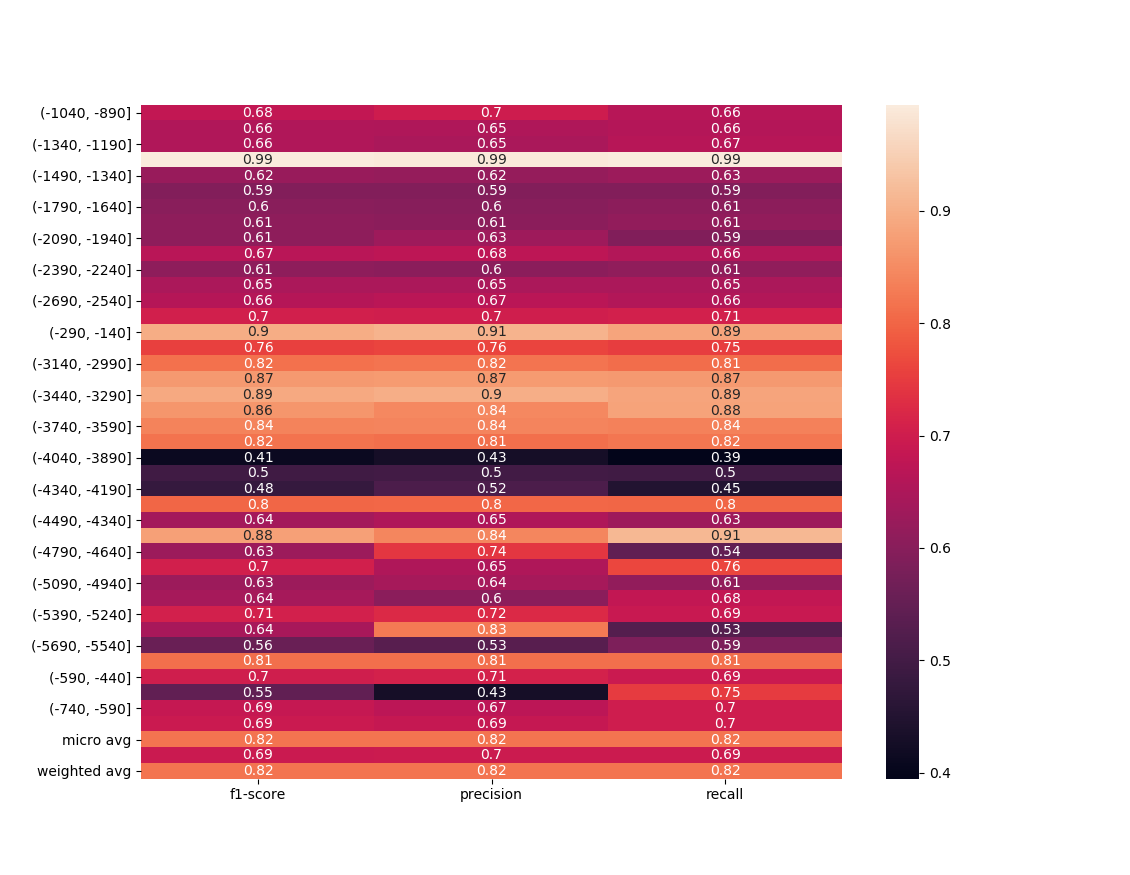
\includegraphics[width=\textwidth]{rfc_class_report.png}
    \caption{Figure displaying the heat map classification report of the Random Forest Classifier}
    \label{fig:rfc_report}
\end{figure}

\par
Figure \ref{fig:rfc_report} displays the classification report for the Random Forest Classifier along a reduced selection of classes.
Precision and recall are excellent measurements to show the performance of a classifier.
What is intersting in figure \ref{fig:rfc_report} is that the precision and recall differs drastically between classes.
This suggests that a classifier will perform different based on the depth.
It also suggests that other localized factors could impact the decision boundaries as the depths are tied to a physical location.

\subsection{Grid Optimized Model Discussion}
%The world wide ETOPO bathymetry dataset \cite{national1988etopo} at two minute resolution is used for valadation and metrics.
%This dataset is treated as the ground truth for all predictions.
%During the experiment, a one third holdout was used for validation in some cases.
%For finding the optimum model for a coverage a 10 fold cross validation was utilized.

%Include metrics information here.... possibly graphs and a list of scores? I dont really know.

%I dont like how I worded this whole section...
%The idea here is that I want to say "Hey, these people did this research and found the their regression model preforms poorly for predicting seamounts espicially after 500m.
%I clearly noticed a similar trend, but saw better preformance from some models than others. 
%This research is to identify those coverages and then use those results to build a super classifier.
%These metrics are important for identifying where the models preform well. 
\par
The Grid Optimized Model Injector improved the accuracy of predictions by \~{}5\%.
These results are displayed in table \ref{table:GRID_OPT_RESULTS}.
Obviously, the model selection and subsequent injection improved the results of this classifier.
Creating a ensemble of many models and selecting them on demand.
This could be caused by geophysical characteristics that benefit one classifier.
For example, in figure \ref{fig:coveragegrid} the Decision Tree classifier preformed best along what appears to be fault lines.
It is possible that the characteristics related to being in proximity to a fault line benefited the models decision boundary. 

% \begin{table}[htb]
%     \centering
%     \begin{tabular}{|c c c|}
%         \hline
%         \textbf{Model} & \textbf{Average F1 Score} & \textbf{Mean Balanced Accuracy} \\
% 		\hline
% 		Grid Optimized Model Injector & 0.83 & 0.862 \\
% 		\hline
%     \end{tabular}
%     \label{table:GRID_OPT_RESULTS}
%     \caption{Grid Optimized Model Injector Results}
% \end{table}

\par
In any event, there is evidence to support geophysical location drives the factors that help predict bathymetry.
Things to optimize may include investigating the appropriate feature sets, coverage boundaries, depth boundaires, parameters, and metrics based on geophysical location.
For example, volcanic activity creates new land.
This activity has a causal relationship to bathymetry, but volcanic activity at a specific point may not affect the bathymetry at a potential antipotle point.
Another example being that the coverage boundaries are potentially a naive selection choice.
It is possible that chossing models by preformance across depth boundaries proves to be a better selector.
%Extending off the research preformed in \cite{jena2012prediction} these metrics allow the selection of the best preforming model.

%Maybe here I can have a table show casing the preformance of models or possibly statistics about the coverages??
%It will be intersting to see what has preformed better across the globe
%Also is intersting to see which models have preformed best overall.

\subsection{General Discussion}
Talk about some bull jive here brooooo